\chapter{Methods}
\section{Data}\label{data}

\subsection{Dataset}

The dataset for this research comes from the Massachusetts Bay Transportation Authority (MBTA).  The data is publicly available and consists of the following:

\begin{itemize}
  \item GPS data for buses, consisting of latitude, longitude, route, and route direction
  \item Route data, describing the GPS location of stops along a route
  \item Bus timetable information, which shows the times when a bus arrives at each stop in a route
  \item Bus metadata
\end{itemize}

Buses, routes and stops are described by ids.  Bus stops also have human readable names indicating their location.
The dataset spans several years, and includes all of the buses and routes in Boston.
This dataset is unique from previous research in its extent both in size and duration.
Previous studies use several months of data, whereas this dataset allows the analysis of longer term trends, including seasonal trends.

Figure~\ref{gps} shows GPS data for Route 1.  The route starts in Cambridge at Massachusetts Avenue and Holyoke Street, and ends in Boston at Dudley Station.
The GPS data is fairly accurate for the most part.
However, in cities like Boston, GPS data suffers from an issue known as urban canyons.
This occurs on relatively narrow streets with very tall skyscrapers, where a canyon effect is created.
The large buildings obscure satellite signals, creating very noisy GPS signals.
Certain streets in Boston suffer from this issue, however Route 1 does not touch those streets, resulting in relatively clean GPS data.
All of the data points are well localized to the street.

\begin{figure}
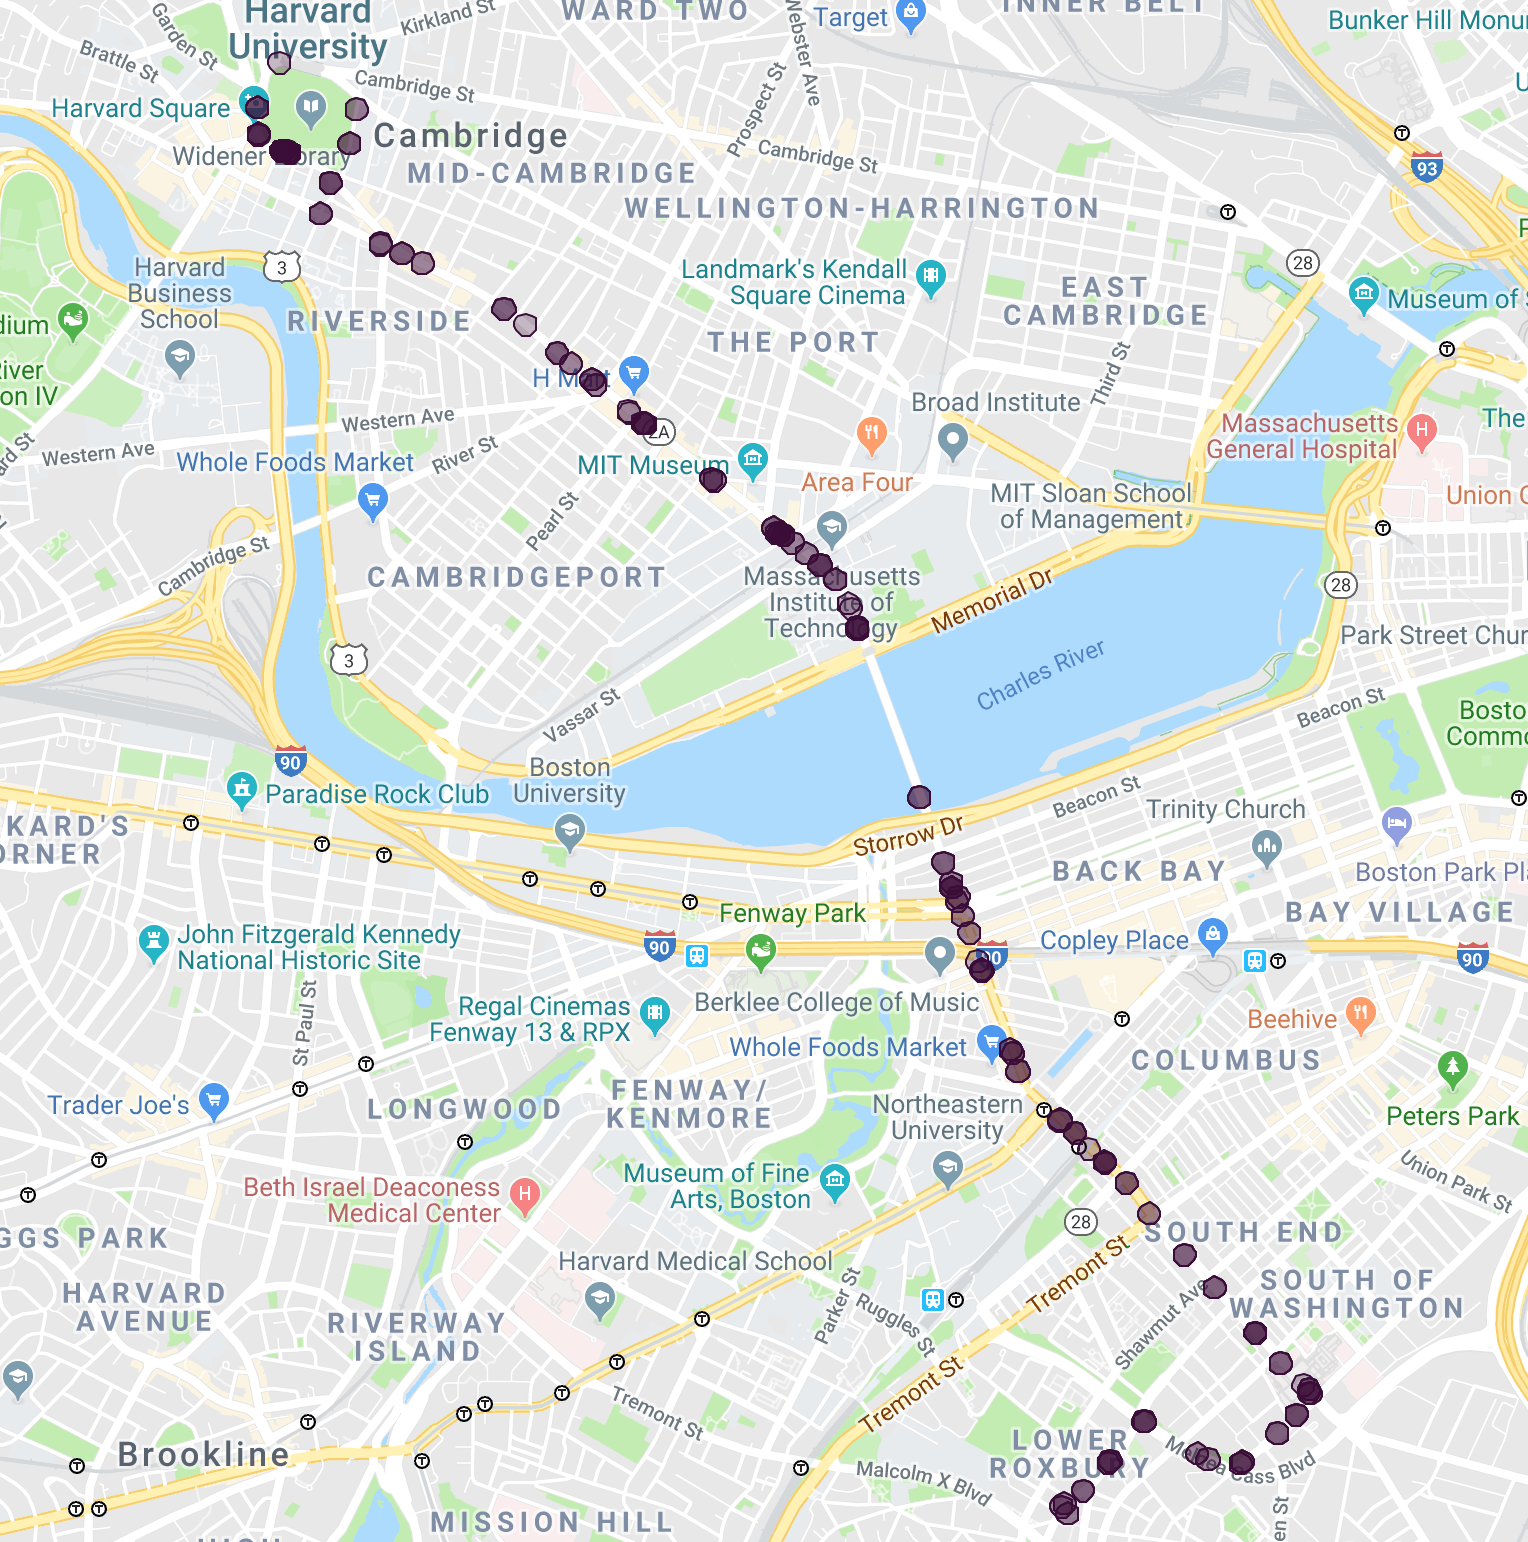
\includegraphics[width=\linewidth]{images/map.png}
%\vspace{2.4in}
\caption{GPS Data from Route 1 serving Cambridge and West Boston}
\label{gps}
\end{figure}
\clearpage
\newpage

\subsection{Interpolating Trajectories}

The data provided consists of tuples of latitude, longitude, bus id, and timestamp.
However, the data needed to train the model involves the arrival times at each stop, so the trajectory of the bus must be interpolated from the noisy GPS data.
This is done via the following process:

\begin{enumerate}}
\item Tuples are grouped by bus id and route, then sorted in time
\item The GPS trajectory is then converted from latitude and longitude into a 2D Cartesian projection
\item The entire trajectory of the bus is segmented into each individual trip along the route
\item The 2D coordinates are then projected onto the route using a Gaussian noise assumption, shown in Figure~\ref{path}
\item This (x,y,t) data is the converted from a 2D position on the map to a 1D distance along the route, because all buses follow the same route
\item Stop data of the form (latitude, longitude) is then converted into the same 1D distance along the path.
\item The trajectory of the bus is then interpolated in a piecewise linear fashion, assuming a constant speed between adjacent points.
\item The trajectory is sanitized by removing any erroneous data by thresholding the velocity of the vehicle
\item This trajectory can then be used to determine the arrival time at each stop by determining the timestep when each bus was within a certain threshold of the stop. This is illustrated in Figure~\ref{interpolate}.
\end{enumerate}}

\begin{figure}
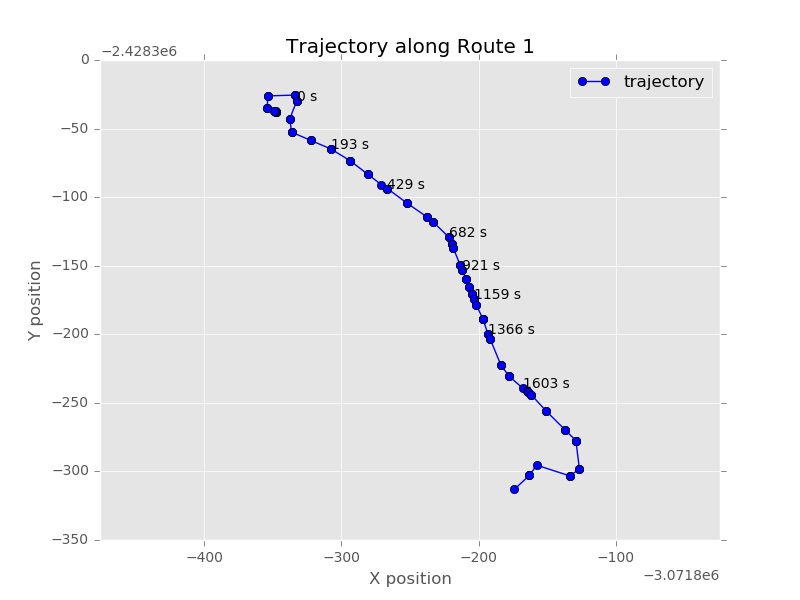
\includegraphics[width=\linewidth]{images/path.png}
%\vspace{2.4in}
\caption{(x,y,t) trajectory of bus along route 1. The routes starts on the top left and finishes on the bottom right.}
\label{path}
\end{figure}
\clearpage
\newpage

\begin{figure}
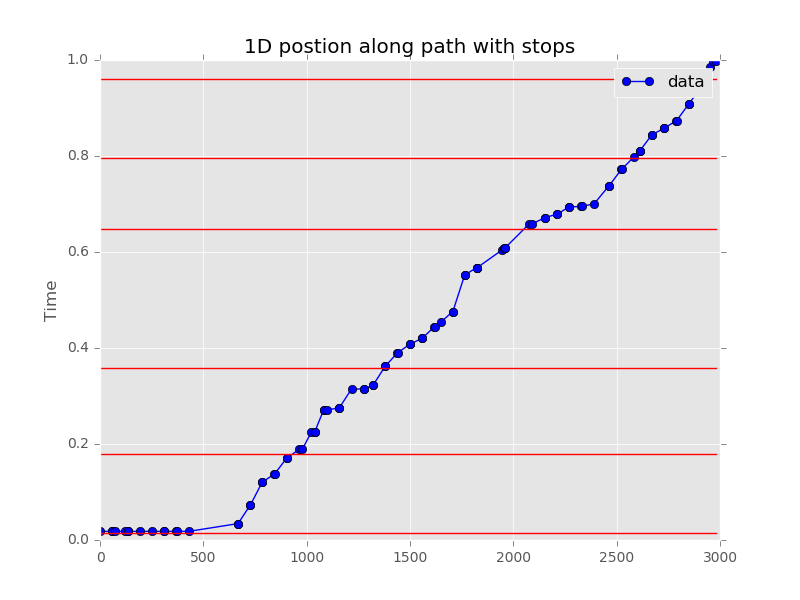
\includegraphics[width=\linewidth]{images/interpolate.png}
%\vspace{2.4in}
\caption{Interpolated trajectory of bus (blue) with stop locations overlain (red). Intersections indicate the bus arriving at a stop.}
\label{interpolate}
\end{figure}
\clearpage
\newpage

\subsection{Features}

The following are a number of features which are commonly used as variables to model bus networks.

\begin{itemize}
  \item Arrival Time: Time the bus arrives at a stop
  \item Travel Time: Between each stop
  \item Dwell Time: The amount of time a bus spends at a stop
  \item Schedule Adherence: The difference between the projected arrival time and the actual arrival time
  \item Headway: The difference in arrival time for two adjacent buses at a specific stop
  \item Direction: For a route which runs two both directions
  \item Weather
  \item Traffic Congestion
  \item Day of Week
  \item Month of Year
\end{itemize}

The arrival time at each stop is computed as shown above.
Travel time can them be trivially computed by taking the difference between two arrival times, minus the dwell time.
Schedule adherence is computed by comparing the arrival time of the bus the closest listed arrival time.
Other features are either derived from the raw data or pulled from outside sources.

\subsection{Distribution of Arrival Times}

Figure~\ref{dist} is a histogram of the difference in arrival times between adjacent buses at a particular stop on Route 1.
Three plots are overlain on the distribution.
If the buses ran perfectly on schedule, the distribution should be concentrated about the mean, indicated by the dotted black line.
If the buses are perfectly random and independent, the distribution should follow a Poisson distribution, indicated in green.
However buses are not independent.
In particular, a bus will not pass another bus, which leads to the high concentration about zero in the distribution.
This effect is compounded by bus clumping.
The exponential distribution captures the behavior of the buses near the origin.
More complicated distribution like the GUE have been used to describe intervals between buses.
A study out of Cuernavaca, Mexico \cite{baik2006model} first identified this effect, and the same effect is observed in the New York public transit system.

\begin{figure}
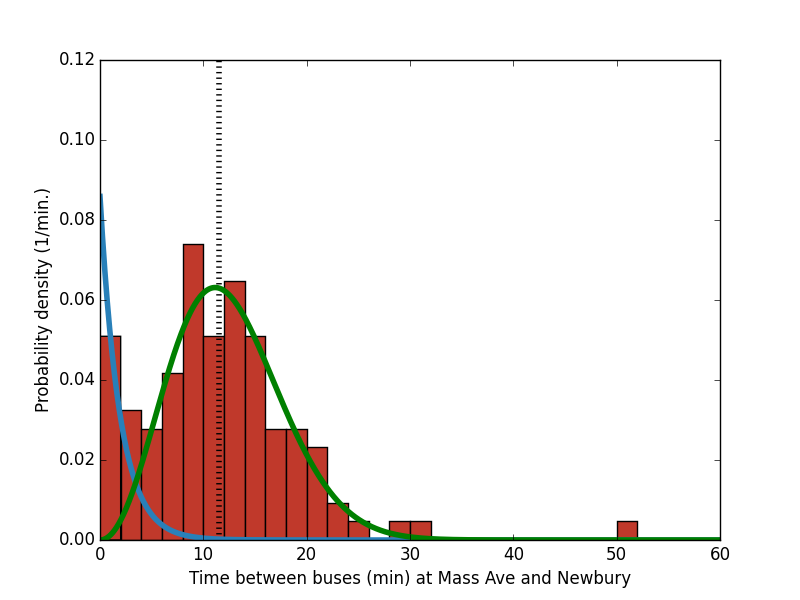
\includegraphics[width=\linewidth]{images/dist.png}
%\vspace{2.4in}
\caption{Distribution of intervals between bus arrival times at Newbury and Mass. Ave.}
\label{dist}
\end{figure}
\clearpage
\newpage

\section{Implementation}

All of the models were developed in Julia \cite{bezanson2012julia} using Knet \cite{yuret2016knet}.
Knet is a declarative machine learning library which supports automatic differentiation and GPUs.
Models are expressed in pure Julia code, then auto-diff is used to generate gradients which can used to train the model.
Several optimizers including stochastic gradient descent, RMSprop and Adam are implemented, as well as many common utility operations and layers.

\section{Models}\label{models}

Three model architectures were used to predict bus arrival times:

\begin{itemize}
  \item Multilayer Perceptron (MLP)
  \item Convolutional Neural Network (CNN)
  \item Recurrent Neural Network (RNN)
\end{itemize}

All three models are applied in regression mode, taking as input knowledge of the bus network, and outputting the expected arrival time at future stops.
Each of the three architectures is successful in predicting arrival times, with the RNN achieving the highest accuracy.

\subsection{Multilayer Perceptron}

Multilayer perceptrons, also known as vanilla neural networks, are the most basic neural network architecture.
They consist of a series of dense linear transformations followed by element-wise non-linear transformations.
Each of these steps is known as a fully connected layer, because at each layer, neurons are connected via a weight matrix to every neuron in the next layer.
Popular non-linear transformations include the sigmoid, hyperbolic tangent, and rectified linear (ReLU).
Figure~\ref{relu} shows the function of a single ReLU.

\begin{figure}
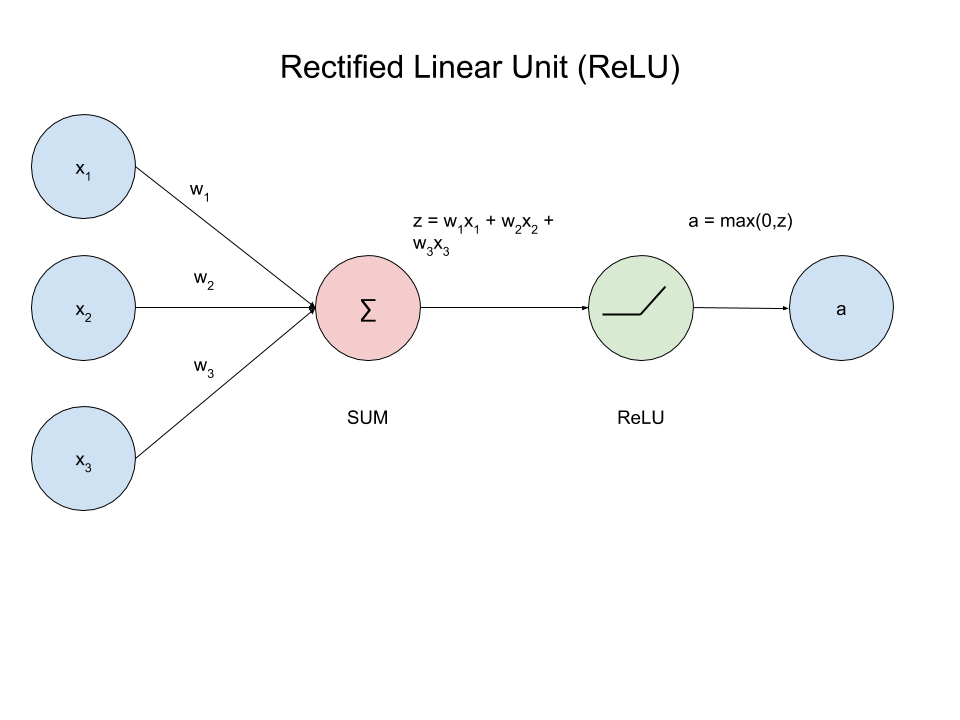
\includegraphics[width=\linewidth]{images/relu.png}
%\vspace{2.4in}
\caption{Rectified Linear Unit}
\label{relu}
\end{figure}
\clearpage
\newpage

The architecture used in this research uses a relatively small neural network with two hidden layers, shown in figure~\ref{mlp_architecture}.
The number of neurons used in each layers was 15 and 10.
This small model size was used to combat overfitting.
The model was trained using a mean squared error loss function for 50 epochs, with a learning rate of 0.0001.
The optimizer used was stochastic gradient descent.
Mean square loss is suitable for most regression tasks.

\begin{figure}
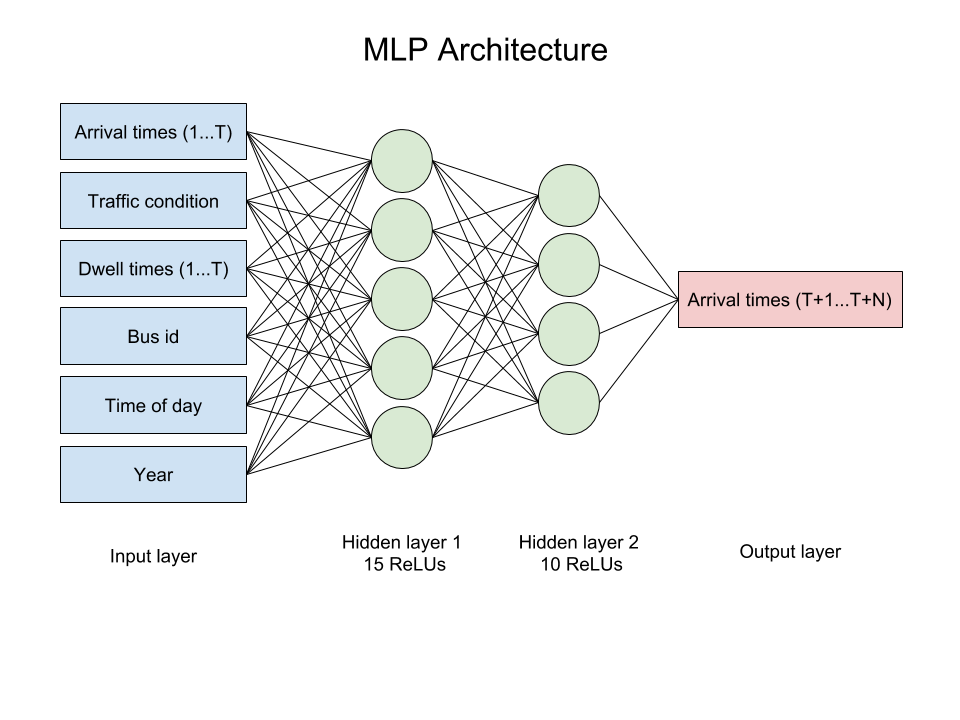
\includegraphics[width=\linewidth]{images/mlp_architecture.png}
%\vspace{2.4in}
\caption{Multilayer Perceptron Architecture: Two fully connected hidden layers}
\label{mlp_architecture}
\end{figure}
\clearpage
\newpage

The following is the code which implements the MLP.

\begin{lstlisting}
# w is a vector of weight matrices
# x is the input vector
function mlp(w,x)
    for i=1:2:length(w)
        # Apply linear transformation
        x = w[i]*x .+ w[i+1]
        if i<length(w)-1
            # Apply ReLU non-linearity
            x = max.(0,x)
        end
    end
    return x
end
\end{lstlisting}

\subsection{Convolutional Neural Network}

Convolutional neural networks are used primarily for image classification, where convolutional filters are applied iteratively to an image to detect low and high level features in the image.
However they are also applicable to regression tasks.
For time series prediction, 1D convolutions are used, as opposed to the 2D convolutions applied to image tasks.
1D convolutions are therefore suitable for the time series task of predicting bus arrival times.

The architecture used contains two convolutional layers followed by two fully connected layers, shown in figure~\ref{cnn_architecture}.
The first convolutional layers consists of 20 filters with 5 neurons each, and the second filter consists of 5 filters with 5 neurons each.
The number of neurons in the fully connected layers depends on the number of input features and number of stops being predicted.
Again, mean squared error loss was used to train the model.

\begin{figure}
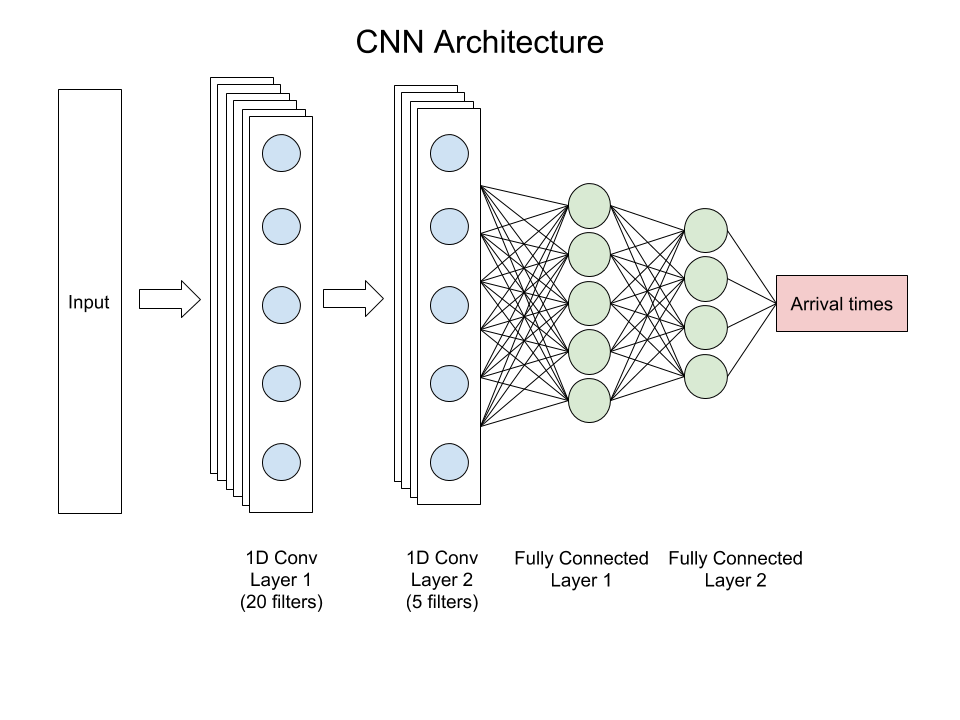
\includegraphics[width=\linewidth]{images/cnn_architecture.png}
%\vspace{2.4in}
\caption{Convolutional Neural Network Architecture: Two convolutional layers and two fully connected hidden layers}
\label{cnn_architecture}
\end{figure}
\clearpage
\newpage

The following is the code which implements the CNN.

\begin{lstlisting}
# w is a vector of weight matrices
# x is the input vector
function cnn(w,x)
  x = reshape(x,(length(x),1,1,1))
  n = length(w)-4
  for i=1:2:n
    # Apply a convolution with max pooling
    x = pool(max.(0, conv4(w[i],x) .+ w[i+1]))
  end
  # Flattens the vector before the fully connected layers
  x = mat(x)
  for i=n+1:2:length(w)-2
    # Apply linear transformation and ReLU activation
    x = max.(0, w[i] * x .+ w[i+1])
  end
  return w[end-1] * x .+ w[end]
end
\end{lstlisting}

\subsection{Recurrent Neural Network}

Recurrent neural networks (RNNs) extend feed forward neural networks such as CNNs and MLPs by adding persistent state.
Typically RNNs are used to model sequences, with the internal state of the network being updated as the sequence is fed through it.
This makes them particularly well suited for time series analysis.

This research uses an Elman network with a hyperbolic tangent activation\cite{elman1990finding}.
The network used consists of a single hidden layer with 10 recurrent neurons.
In each time step, a single element of the input sequence is fed into the network, producing an output and a hidden state.
The output is used to train the network, and the hidden state is fed into the network on the next timestep.
This is illustrated in figure~\ref{rnn_architecture}.
The network is fed some empty initial state, in this case a zero vector.

\begin{figure}
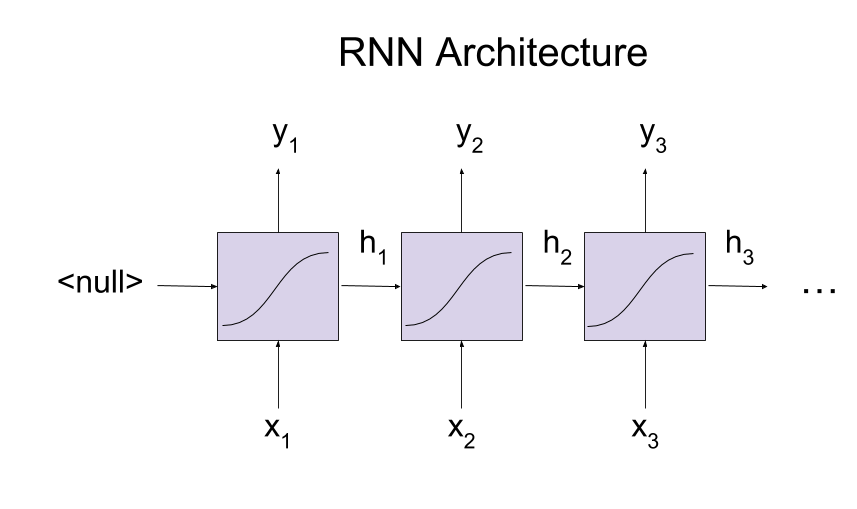
\includegraphics[width=\linewidth]{images/rnn_architecture.png}
%\vspace{2.4in}
\caption{Recurrent Neural Network Architecture: One hidden layer with 10 neurons}
\label{rnn_architecture}
\end{figure}
\clearpage
\newpage

The network was trained via back propagation through time (BPTT)\cite{WERBOS1988339}.
This allows for training the network across an entire sequence, and reinforcing the correct outputs at each step of the sequence.
Again, root mean square error across the predictions was used as the loss function.

The following is the code which implements the RNN in Julia.

\begin{lstlisting}
# w is a vector of weight matrices
# x is the input vector
# h is the state
function rnn(w,x,h)
    # Generate the new state from the previous state and the input
    h = tanh.(w[1]*vcat(x,h) .+ w[2])
    # Generate prediction from state
    y = w[3]*h .+ w[4]
    return (y,h)
end
\end{lstlisting}
